\Chapter{Részszámítások elemzése}

\Section{Beolvasási idők vizsgálata}

Azoknál a módszereknél, amelyek mért futásidejében jelentős különbség adódott a C-s, illetve a Rustos implementáció között van egy közös jellemzőjük: nagyméretű inputot olvasnak be fájlból. Így adódik a felvetés, hogy a fájl beolvasáshoz szükséges idő jelenti a differenciát a két implementáció között.

\Aref{fig:file}. grafikonon látható, hogy Rustban a beolvasás jóval lassabb, a futásidők különbségét magyarázza.

\begin{figure}[h!]
\centering
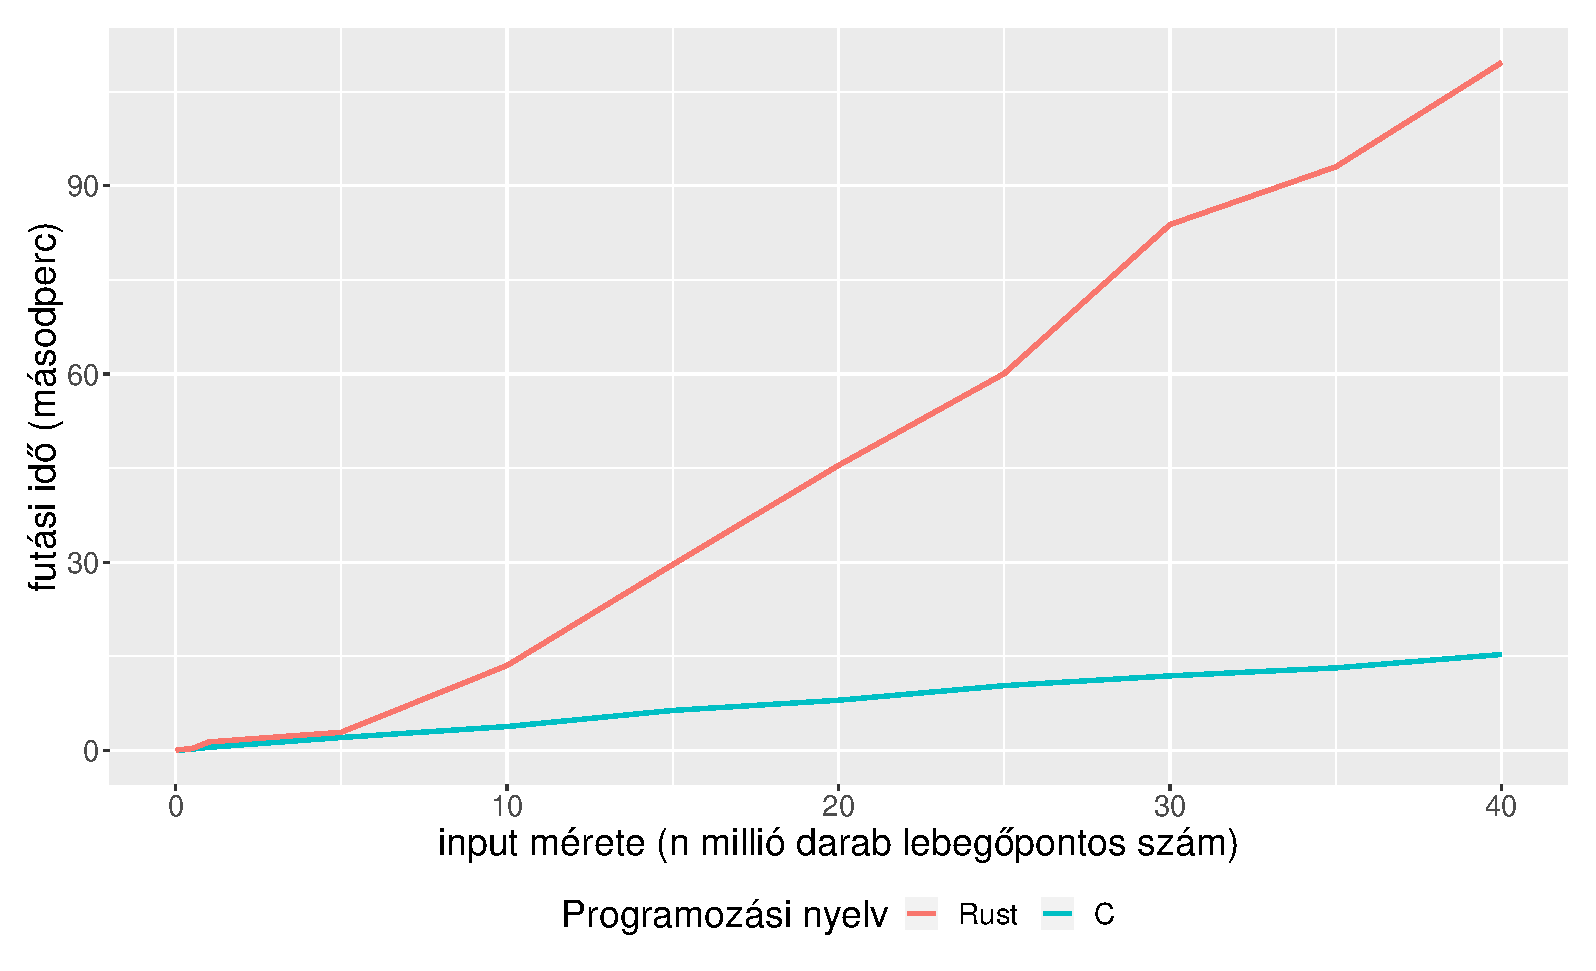
\includegraphics[width=15.5cm]{kepek/file_read.eps}
\caption{A fájlbeolvasás időigénye a három implementáció esetén}
\label{fig:file}
\end{figure}

\SubSection{Futásidők a fájl beolvasása nélkül}

A következőkben azt láthatjuk, hogy hogy változnak az egyes algoritmusok futási idejei, hogy ha a fájlbeolvasást egy független műveletnek tekintjük, és a már elérhető adatszerkezeten végezzük el a számításokat.

\subsubsection{Kupacrendezés}

A kupacrendezés futási idejét \aref{fig:heap_fixed}. ábrán láthatjuk.

\begin{figure}[h!]
\centering
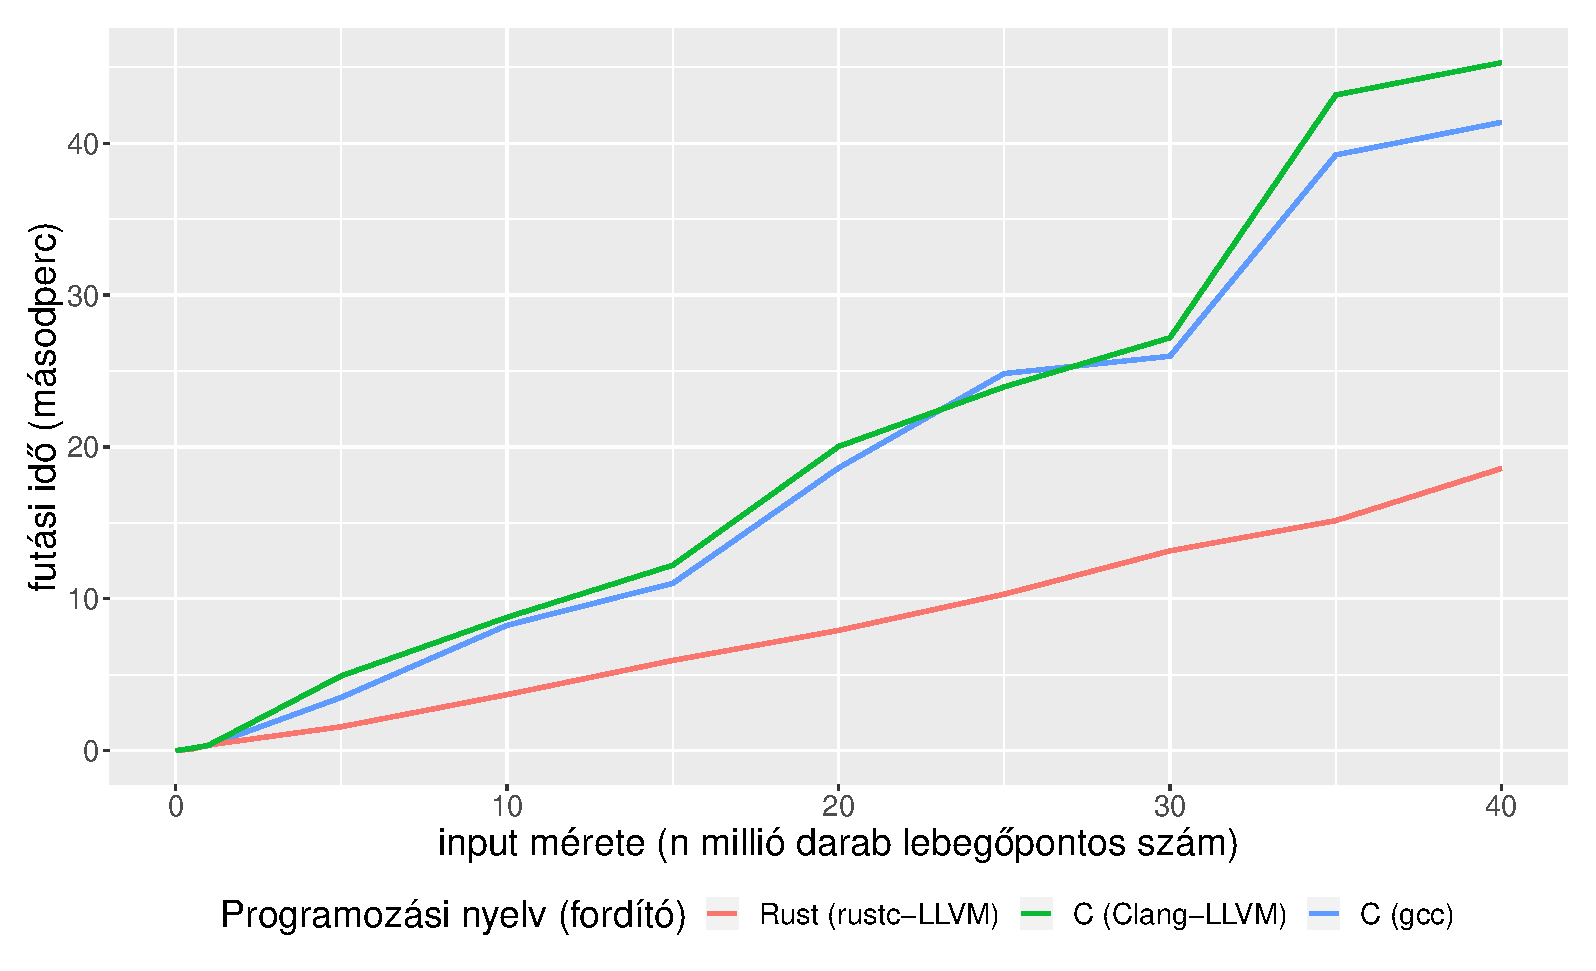
\includegraphics[width=15.5cm]{kepek/heap_sort_run_without_read.eps}
\caption{A kupacrendezés futási ideje}
\label{fig:heap_fixed}
\end{figure}

Ebből az látható, hogy a Rust-nak így már jelentős előnye van a C nyelvű implementációkhoz képest.

\subsubsection{Shell-rendezés}

A Shell-rendezés esetében is jelentősen javultak a számítási idők a Rust-ra nézve (\ref{fig:shell_fixed}. ábra). A GCC és CLang implementációk között jelentős különbség itt sem látható.

\begin{figure}[h!]
\centering
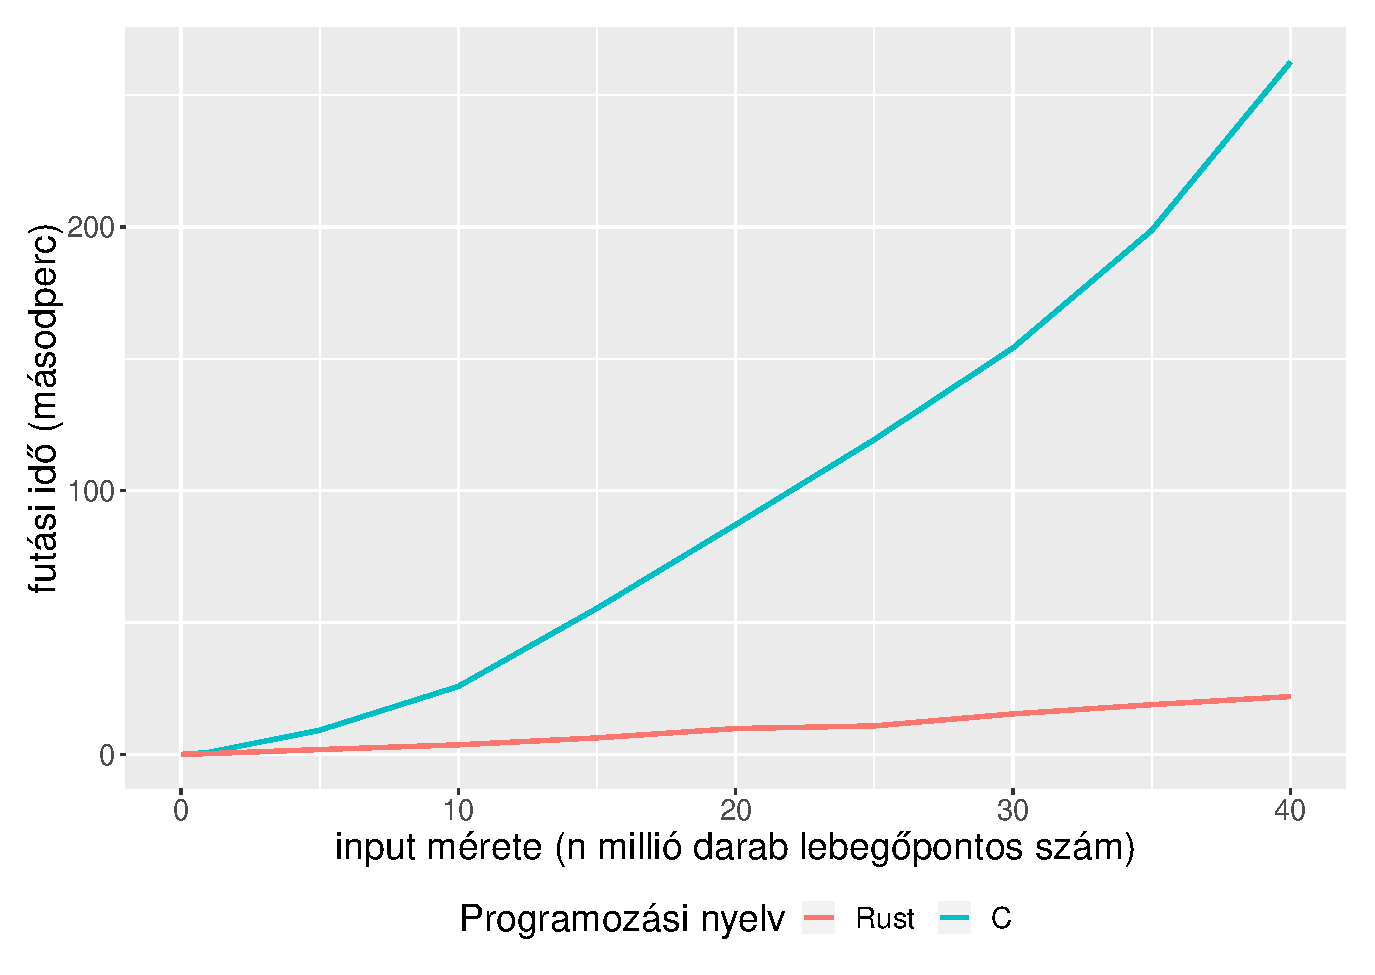
\includegraphics[width=15.5cm]{kepek/shells_sort_run_without_read.eps}
\caption{A Shell-rendezés futási ideje}
\label{fig:shell_fixed}
\end{figure}

\subsubsection{Gyorsrendezés}

A gyorsrendezés esetében a számítási idő tulajdonképpen kiegyenlítődött, de a tendencia azt mutatja, hogy a Rust a leggyorsabb, amelyet a CLang majd a GCC követ (\ref{fig:quicksort_fixed}. ábra).

\begin{figure}[h!]
\centering
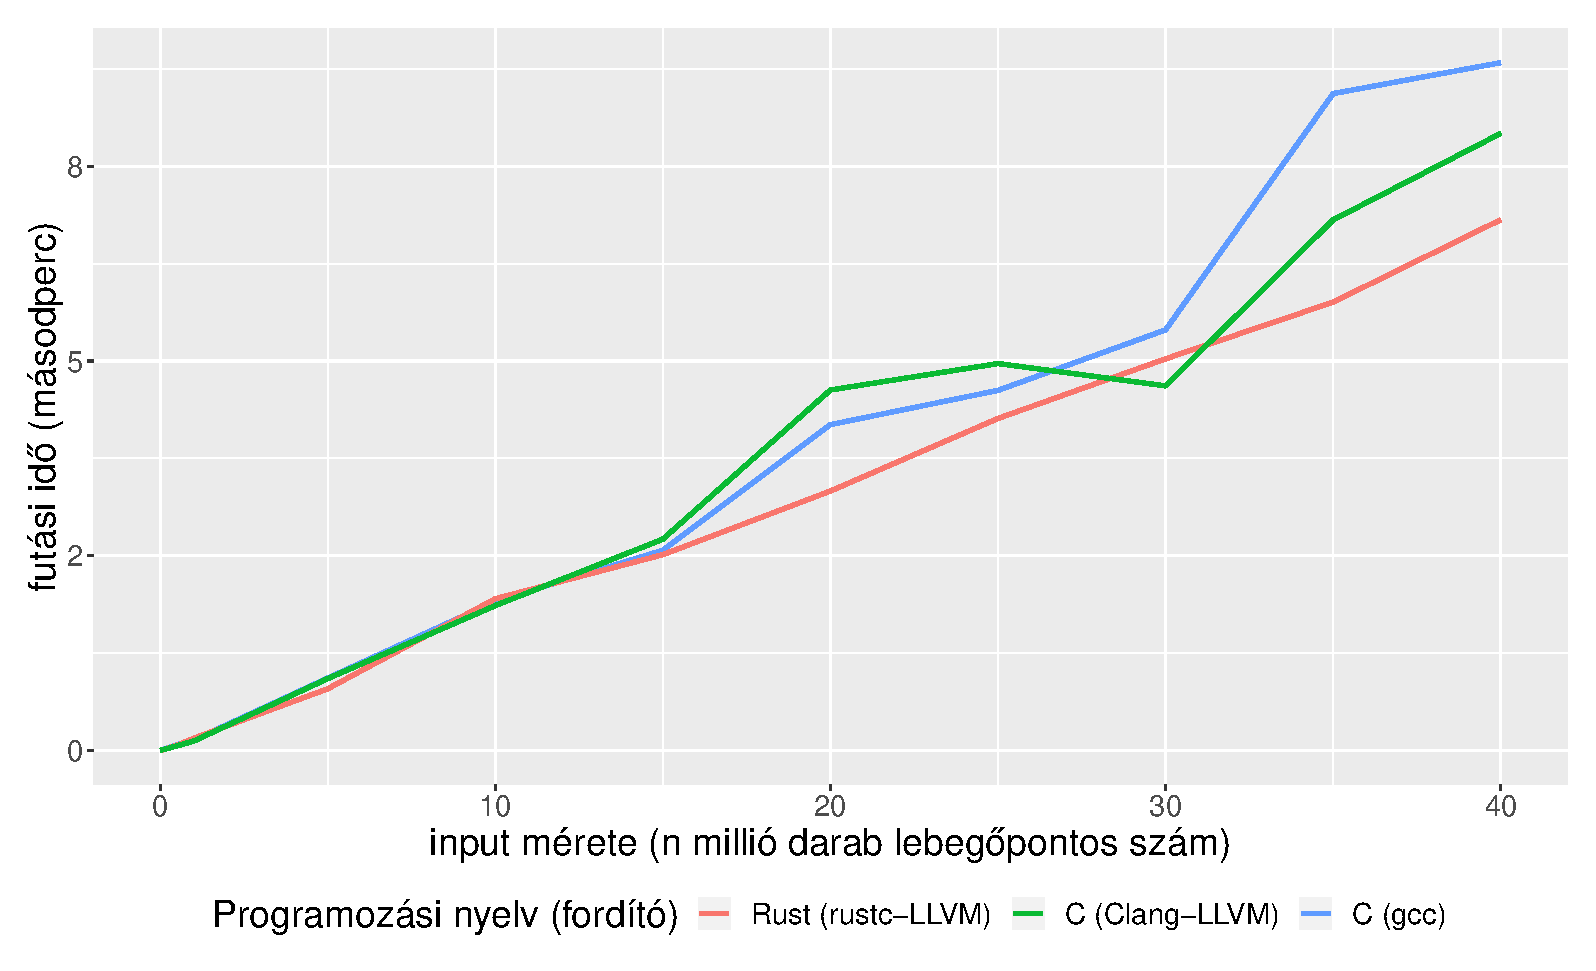
\includegraphics[width=15.5cm]{kepek/quicksort_run_without_read.eps}
\caption{A gyorsrendezés futási ideje}
\label{fig:quicksort_fixed}
\end{figure}

\subsubsection{Lineáris interpoláció}

A lineáris interpoláció esetében is futási idő a Rust változatban volt a leggyorsabb. A gyorsrendezéssel ellentétben itt a GCC-s implementáció mutatkozott jobbnak az LLVM-eshez képest.

\begin{figure}[h!]
\centering
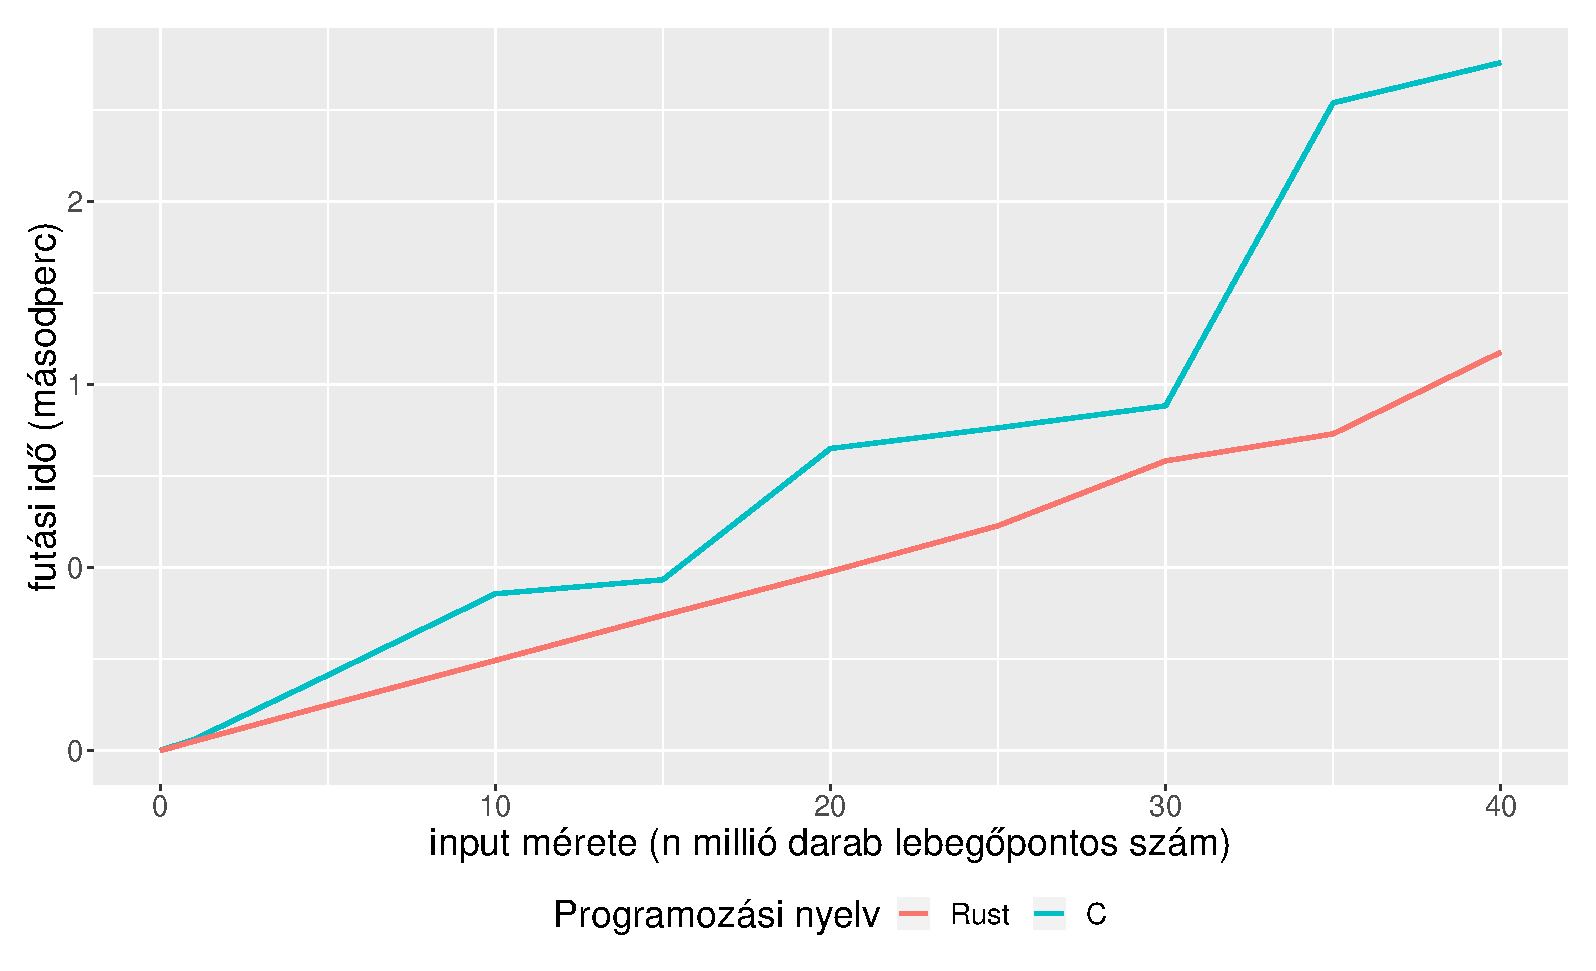
\includegraphics[width=15.5cm]{kepek/linear_interpolation_run_without_read.eps}
\caption{A lineáris interpolációs számítás futási ideje}
\label{fig:interpolation_fixed}
\end{figure}

Látható tehát, hogy maga a módszer a Rust implementációban minden esetben gyorsabb, ha az inputfájlok beolvasását nem mérjük, tehát nem tekintjük a megoldandó számítási feladat részének.
